\section{Locomotion}
\label{sec:Locomotion}
Soft and continuously deformable locomotion systems can be made from bending fluidic elastomer segments.
Specifically, in this section we detail how soft robotic fish can be composed by combining the actuated segments that were presented in Section~\ref{subsec:Actuators, Actuator Morphologies} with a portable power system.

\subsection{Pneumatic Fish}
\label{subsec:Locomotion, Pneumatic Fish}

%\begin{figure}[htb]
%        \centering
%        \begin{subfigure}[b]{\columnwidth}
%            \centering
%            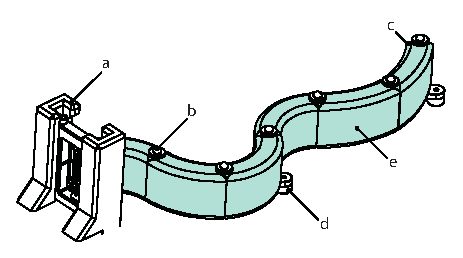
\includegraphics[width=0.9\columnwidth]{Figures/manipulators/ribbed_manipulator}
%            \caption{}
%            \label{fig:ribbed_manipulator_design}
%        \end{subfigure}\\
%        \begin{subfigure}[b]{\columnwidth}
%            \centering
%            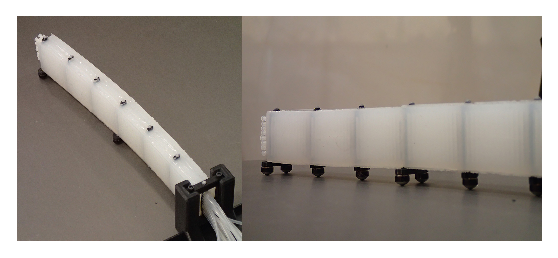
\includegraphics[width=0.9\columnwidth]{Figures/manipulators/ribbed_manipulator_real}
%            \caption{}
%            \label{fig:ribbed_manipulator_real}
%        \end{subfigure}%
%        \caption[A ribbed soft manipulator prototype.]{A ribbed soft manipulator prototype. (\textbf{a}) The arm is composed of homogeneous and independently actuated ribbed segments (e). The base of the arm's first segment is fixed (a) and the end of its last segment is the end-effector (c). Markers (b) identify the endpoints of each segment and ball transfers (d) mitigate friction. (\textbf{b}) Photographs of the ribbed manipulator prototype.}
%\end{figure}

\subsection{Hydraulic Fish}
\label{subsec:Locomotion, Hydraulic Fish}

%\begin{figure}[htb]
%\centering
%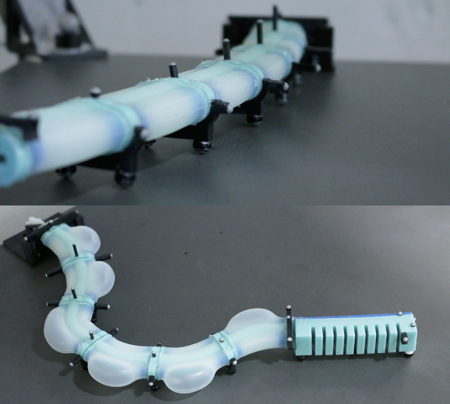
\includegraphics[width=\columnwidth]{Figures/manipulators/cylindrical_manipulator_real}
%\caption[A cylindrical soft manipulator prototype.]{A cylindrical soft manipulator prototype with and without a pleated finger-like gripper.} \label{fig:cylindrical_manipulator}
%\end{figure}
